\section{Manual}
In the following section the most important functionalities of the votes system are summarized.

\subsection{Login}

The Votes login page displayed in figure \ref{F:votes_login} is the entry-point to the system. A direct login is possible by entering an already registered email address an the correct password to the account. If no account has been created the user can sign in by first select \textit{Register} in the menu appearing when clicking on the top right button. If the resolution of the browser is high the menu is replaced by buttons in the black top bar. Clicking the \textit{Register} button is followed by the registration page. A valid account requires a \textit{Username}, \textit{Realname}, \textit{Email} and \textit{Password}.

\begin{figure}
\centering
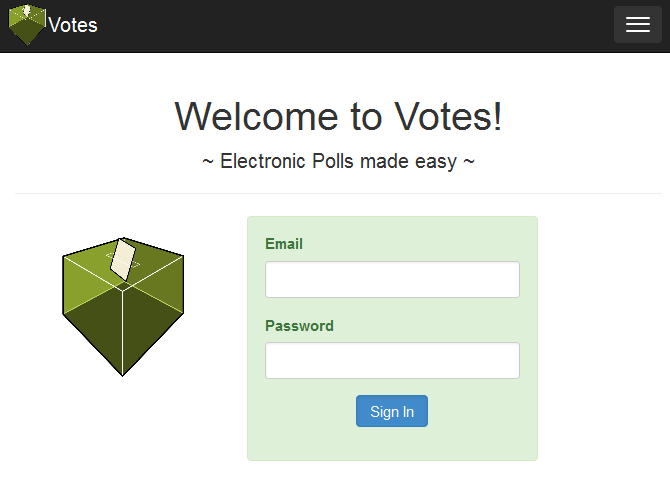
\includegraphics[width=0.4\textwidth]{png/votes_login.png}
\caption{Votes login page}
\label{F:votes_login}
\end{figure}

\subsection{Browse my Polls}
When logged in the \textit{My Polls} page, displayed in figure \ref{F:browse_my_polls}, appears. Here all \textit{Polls} and some poll properties can be viewed on one single page. For informations that go deeper into the \textit{Polls} data the \textit{Poll} has to be clicked. The table displays title, state and results. The results can only be viewed when available.

\begin{figure}
\centering
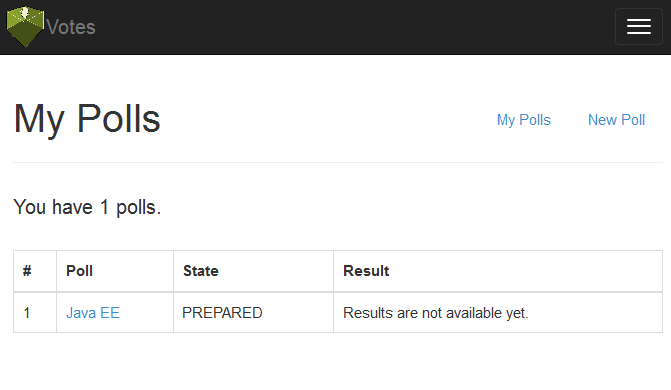
\includegraphics[width=0.5\textwidth]{png/browse_my_polls.png}
\caption{Top part of the Votes \textit{Edit Poll} page}
\label{F:browse_my_polls}
\end{figure}



\subsection{Create and edit Polls}

\textit{Polls} can be created by pressing the \textit{New Poll} button that is located on the upper left corner of every page. By pressing \textit{New Poll} the user gets to a form were an initial \textit{Title} and \textit{Description} have to be entered. After that the user gets to the \textit{Edit Poll} page that can also be entered form the \textit{My Polls} page when selecting an existing poll.

\begin{figure}
\centering
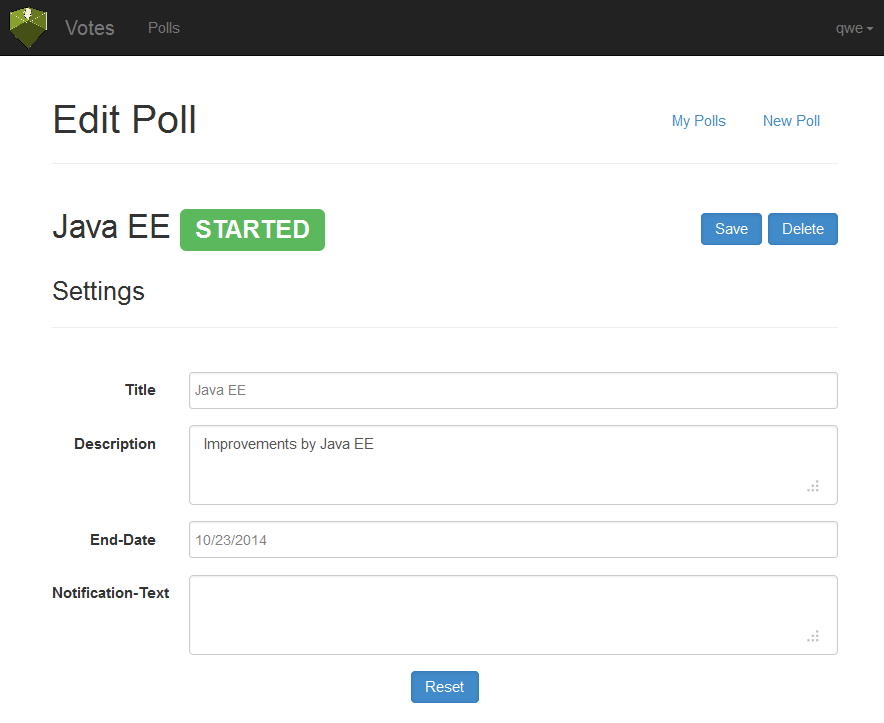
\includegraphics[width=0.5\textwidth]{png/edit_poll.png}
\caption{Upper part of the Votes 'Edit Poll' page}
\label{F:edit_poll}
\end{figure}

The first part of the \textit{Edit Poll} page can be seen in figure \ref{F:edit_poll}. In this case it shows the concrete Poll with the title 'Java EE'. In the four text fields the \textit{Title}, \textit{Description}, \textit{End-Date} and \textit{Notification-Text} can be set. If \textit{Save} is pressed the setting are stored. The \textit{Delete} button deletes the poll. The appearance of the buttons \textit{Reset} and \textit{Start} are dependent on the state of current \textit{Poll}. In figure \ref{F:edit_poll} the \textit{Poll} has the state \textit{Started}, displayed next to the current \textit{Title} in the heading. In this case only the \textit{Reset} button is displayed.  

\begin{figure}
\centering
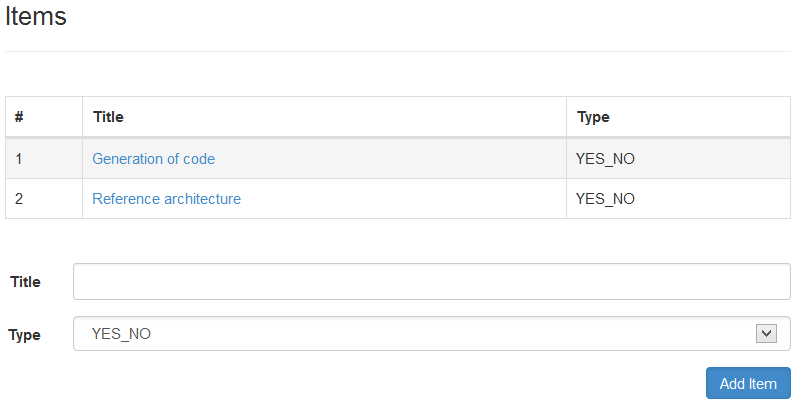
\includegraphics[width=0.5\textwidth]{png/items.png}
\caption{Middle part of the Votes \textit{Edit Poll} page displaying the items of the corresponding poll}
\label{F:items}
\end{figure}

In the middle part of the \textit{Edit Poll} page the list of \textit{Items} belonging to this \textit{Poll} can be edited. This is shown in figure \ref*{F:items}. If the \textit{Poll} is not already in the state \textit{Started}, the user has the option to add an \textit{Item} to the list by pressing the \textit{Add Item} button. The \textit{Title} and \textit{Type} fields are used for the creation of the new \textit{Item}. The possible Types are \textit{YES NO},\textit{ONE OF N} and \textit{M OF N}. All \textit{Items} can be opened by clicking on them in order to modify the \textit{Options}, the \textit{Title} or the \textit{Type}. The opportunity the add, remove or modify \textit{Options} is only given for the \textit{Items} of the \textit{Type} \textit{ONE OF N} and \textit{M OF N}.

\begin{figure}
\centering
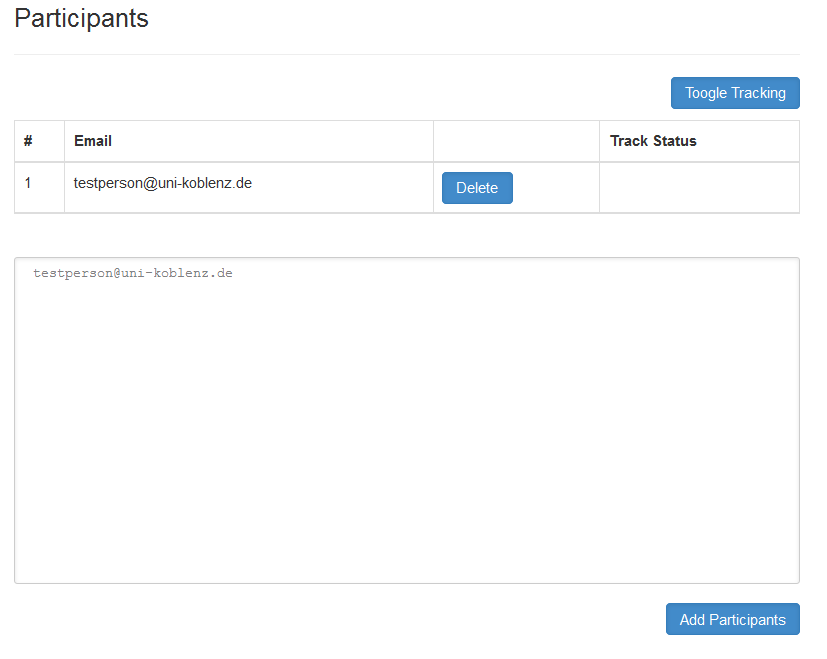
\includegraphics[width=0.5\textwidth]{png/participants.png}
\caption{Bottom part of the Votes \textit{Edit Poll} page displaying the participants of the \textit{Poll}}
\label{F:participants}
\end{figure}

In the bottom part of the \textit{Edit Poll} page, displayed in figure \ref*{F:participants}, participants can be added and removed for the current poll. This is done by writing all mail addresses into the text field and pressing the \textit{Add Participants} button. When the Poll is started the all persons in the list are informed.

\subsection{Vote by using a Token}

\begin{figure}
\centering
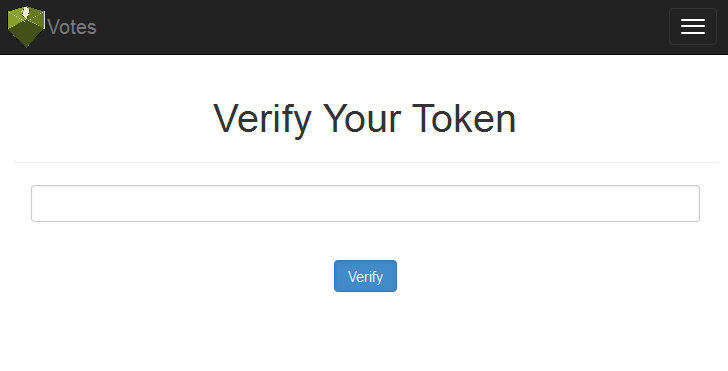
\includegraphics[width=0.5\textwidth]{png/token.png}
\caption{Page for entering \textit{Tokens}}
\label{F:token}
\end{figure}

To vote in the system the \textit{Token} that has been sent by mail must be entered into the page displayed in \ref{F:token}. The link to this page is send ahead with the notification mail. If the \textit{Token} is correct the corresponding voting options appear by pressing the \textit{Verify} button.

\subsection{Votes Result}

Until the poll is finished the organizer is not able to view any results (See: \ref{F:not_available}).
When the poll is finished the organizer will get a link which leads him to the result page (See: \ref{F:show_result}).
The result page shows a bar graph for every item (See: \ref{F:result_charts}). The organizer can see the options of each item with their description beside the charts.

\begin{figure}
\centering
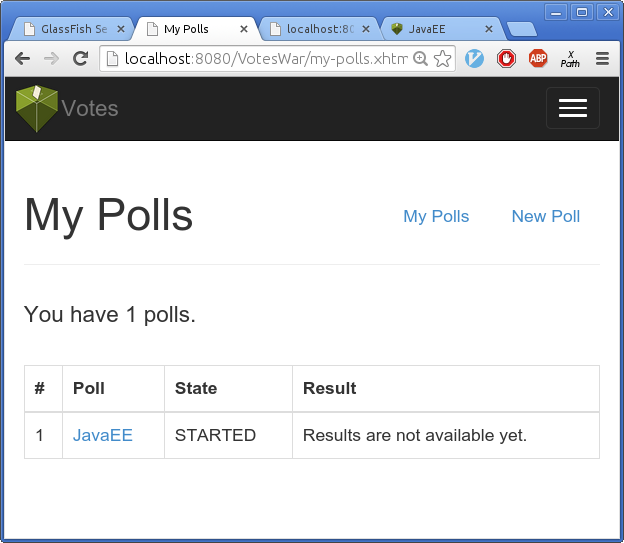
\includegraphics[width=0.5\textwidth]{png/poll_result_not_available.png}
\caption{\textit{Result} not available }
\label{F:not_available}
\end{figure}


\begin{figure}
\centering
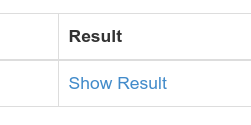
\includegraphics[width=0.5\textwidth]{png/poll_result_show_result.png}
\caption{Poll with \textit{Result} available}
\label{F:show_result}
\end{figure}


\begin{figure}
\centering
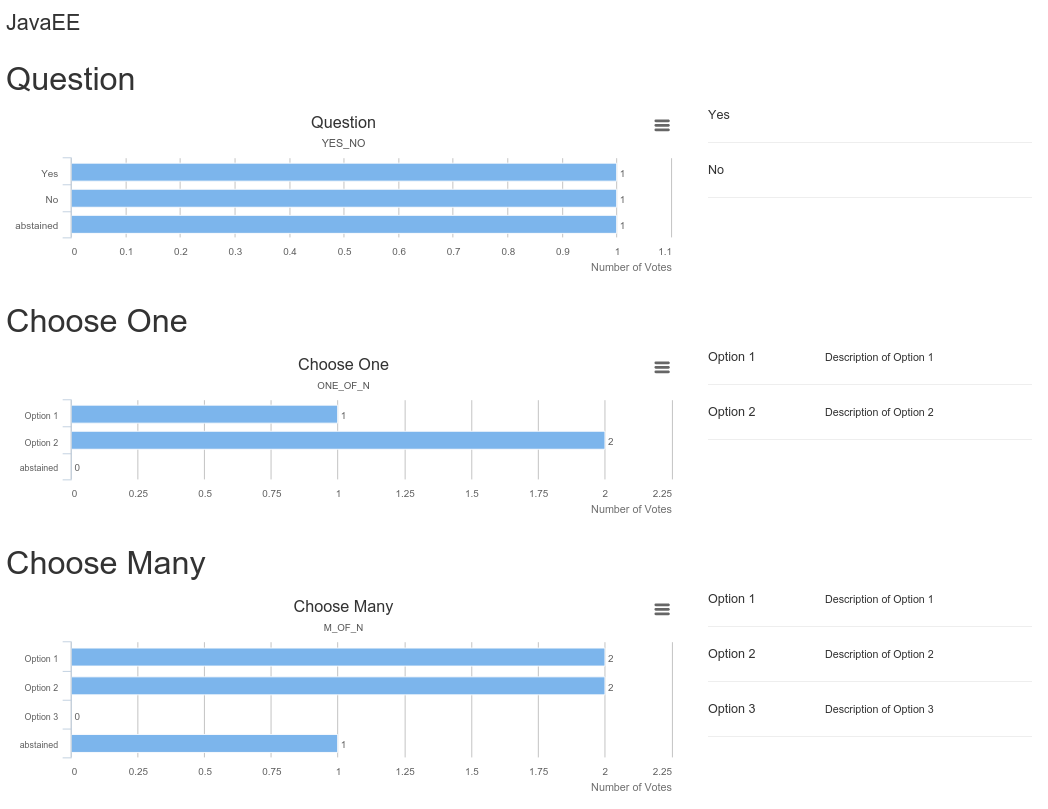
\includegraphics[width=0.5\textwidth]{png/poll_result_view.png}
\caption{Page \textit{Result Charts}}
\label{F:result_charts}
\end{figure}









